% Compiled at build time so the packages most papers load ship with Scientify.
\documentclass[11pt]{article}
\usepackage[T1]{fontenc}
\usepackage[utf8]{inputenc}
\usepackage{lmodern}
\usepackage{geometry}
\usepackage{amsmath,amssymb,amsthm,mathtools,bm}
\usepackage{graphicx}
\usepackage{xcolor}
\usepackage{booktabs,multirow,array,tabularx,makecell,threeparttable}
\usepackage{caption,subcaption,float,wrapfig}
\usepackage{enumitem}
\usepackage{siunitx}
\usepackage{algorithm,algpseudocode}
\usepackage{listings}
\usepackage{tikz}
\usepackage{pgfplots}
\pgfplotsset{compat=1.18}
\usepackage{microtype}
\usepackage[numbers]{natbib}
\usepackage{url}
\usepackage{hyperref}
\usepackage{cleveref}
\usepackage{lipsum}
\newtheorem{theorem}{Theorem}
\title{Warm-up}
\author{Scientify}
\begin{document}
\maketitle
\begin{abstract}
\lipsum[1]
\end{abstract}
\section{Introduction}\label{sec:intro}
See \cref{sec:intro} and \citet{knuth1984}; $\bm{x} = \SI{3}{\metre}$, $\mathbb{R}^n$.
\begin{theorem}
$a^2 + b^2 = c^2$
\end{theorem}
\begin{table}[h]
\centering
\begin{tabular}{lr}
\toprule
Method & Score \\
\midrule
Ours & \num{0.91} \\
\bottomrule
\end{tabular}
\caption{Results}
\end{table}
\begin{algorithm}
\caption{Warm-up}
\begin{algorithmic}
\State $x \gets 1$
\end{algorithmic}
\end{algorithm}
\begin{lstlisting}[language=Python]
print("hello")
\end{lstlisting}
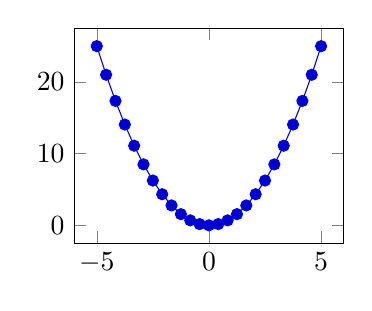
\begin{tikzpicture}
\begin{axis}[width=5cm]
\addplot {x^2};
\end{axis}
\end{tikzpicture}
\textbf{Bold} \emph{emphasis} \texttt{mono} \textsc{Small caps}.
\bibliographystyle{plainnat}
\bibliography{refs}
\end{document}
